%%%%%%%%%%%%%%%%%%%%%%%%%%%%%%%%%%%%%%%%%%%%%%%%%%%%%%%%%%%%%%%%%%%%%%
% How to use writeLaTeX: 
%
% You edit the source code here on the left, and the preview on the
% right shows you the result within a few seconds.
%
% Bookmark this page and share the URL with your co-authors. They can
% edit at the same time!
%
% You can upload figures, bibliographies, custom classes and
% styles using the files menu.
%
%%%%%%%%%%%%%%%%%%%%%%%%%%%%%%%%%%%%%%%%%%%%%%%%%%%%%%%%%%%%%%%%%%%%%%

\documentclass[12pt]{article}

\usepackage{sbc-template}

\usepackage{graphicx,url}

\usepackage[brazil]{babel}   
%\usepackage[utf8]{inputenc}  

\usepackage{comment}
\usepackage{color}
\usepackage{ifthen}
\newcommand{\cl}[1]{\textcolor{red}{\textbf{[Crescencio: #1]}}}
 
 

     
\sloppy

\title{Título do artigo}

\author{Primeiro autor\inst{1}, Crescencio Lima (orientador)\inst{1} }


\address{Instituto Federal de Educação, Ciência e Tecnologia da Bahia (IFBA)\\
   45078-300 -- Vitória da Conquista -- BA -- Brasil
  \email{TBD@gmail.com, crescencio@gmail.com}
}



\begin{document} 

\maketitle

%\cl{Atualizar o abstract de acordo com a nova versão do resumo}
\begin{abstract}
TBD.
\end{abstract}

%\cl{Segue o modelo (template para criar o abstract/resumo: \\ \url{https://blog.fastformat.co/5-passos-resumo-abstract-tcc-normas-abnt/}}
     
%\cl{O resumo deve conter: Contexto, Objetivo, Método(Não se aplica ao nosso trabalho uma vez que não utilizamos nenhum método científico),: Resultados e Conclusões}

\begin{resumo} 
Contexto: TBD.
Objetivo: TBD.
Método: TBD. 
Resultados: TBD.
  
\end{resumo}


\section{Introdução}

TBD.

O restante deste documento está estruturado da seguinte forma: Seção \ref{sec:referencial_teorico} apresenta o referencial teórico da pesquisa. Seção \ref{sec:tecnologias} explica as tecnologias adotadas. Seção \ref{sec:proposta} apresenta o desenvolvimento da proposta. Seção \ref{sec:limitacoes} apresenta as limitações do projeto. Seção \ref{sec:conclusao} explica as conclusões da pesquisa e fala sobre os trabalhos futuros.

\section{Fundamentação Teórica} \label{sec:referencial_teorico}

%\cl{Buscar por referencias principalmente do Simpósio Brasileiro de Sistemas de Informação (SBSI) ou da Revista Brasileira de Sistemas de Informação (iSys).}

%\cl{Na fundamentação teórica é preciso apresentar os conceitos para entendimento do projeto. Por exemplo, acredito que caberia o conceito de CI/CD (Continuous Integration e Continuous Delivery)}

%\cl{Verificar o trabalho de TCC do Wesley (mandei pelo email). Ele fez uma análise dos Sistemas de Informação (SI no contexto de comércio eletrônico (Página 17).}

%\cl{Acho que podemos referenciar o trabalho do  Loh (2014) que descreve que a classificação dos sistemas de informação. Vamos tentar mapear o tipo de sistema do nosso trabalho (Página 23).}



Para se falar de sistemas web, antes é preciso se falar sobre sistemas de informação (SI). ``O objetivo principal de um SI é gerenciar informações, ou seja, coletar, armazenar, organizar, tratar, cruzar, disseminar, gerar e fornecer informações de tal modo a apoiar decisões e processos de uma organização'' \cite[7]{SI}. \cl{Exemplo de citação.}

Um sistema web é um SI hospedado e disponível na internet, o que permite que os usuários utilizem suas funções remotamente, acessando um endereço através de um navegador. Essa característica é fundamental para o objetivo do trabalho proposto.

%\\cl{Tudo que estiver relacionado com comércio eletrônico (foco do trabalho do Wesley), podemos alterar para sistema de gerenciamento de processos seletivos.}

%\\cl{Explicar o que é um sistema de gerenciamento de processo seletivo?}

Um processo seletivo é definido como o ``processo pelo qual alguém tem de passar antes de ser selecionado para uma vaga, geralmente universitária ou laboral; concurso, vestibular'' \cite{processoseletivo}. Analisando os processos da seleção de pós-graduação realizada pelo IFBA para a PGDW, foi possível separar as tarefas executadas em dois grupos, as dos alunos e as dos avaliadores.



%\cl{Como disse no email, HTML, CSS, Javascript, tudo isso pode ir para tecnologia.}




\section{Infraestrutura e Tecnologias} \label{sec:tecnologias}

TBD.

\subsection{Next.js e Vercel}

TBD.

\subsection{Firebase}



Todos esses recursos possuem ainda uma biblioteca nativa para projetos JavaScript, que permite que a realização de consultas, leituras e gravações dos dados e arquivos de forma simples. A Figura \ref{fig:infra1} apresenta a infraestrutura utilizada no projeto. \cl{Exemplo de como citar figura no texto.}



\begin{figure}[ht]
\centering
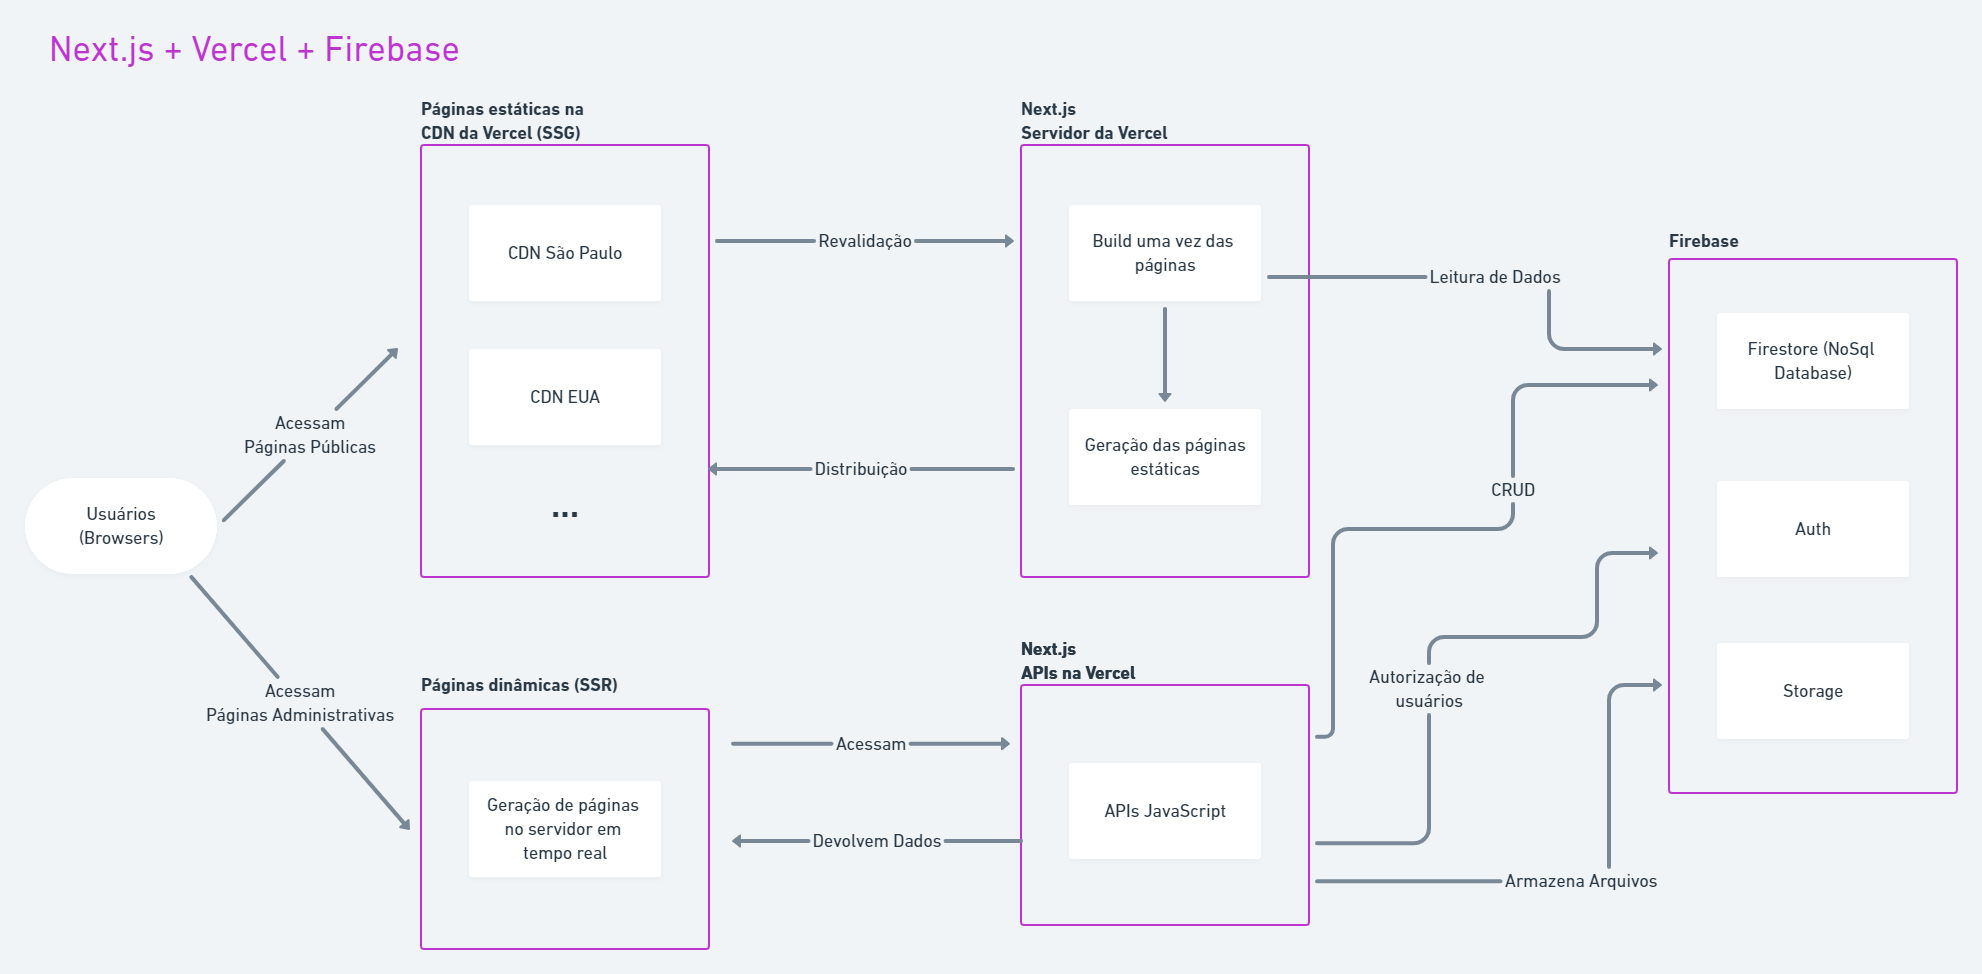
\includegraphics[width=1\textwidth]{imagens/infra.png}
\caption{Infraestrutura \cl{Exemplo de Figura.}}
\label{fig:infra1}
\end{figure}



\subsection{Estrutura dos Dados}

TBD.

\section{Proposta} \label{sec:proposta}

TBD.

\section{Conclusão} \label{sec:conclusao}

TBD.

\bibliographystyle{sbc}
\bibliography{sbc-template}

\end{document}
